\iffalse
	\chapter{2011}
	\author{AI24BTECH11003}
	\section{xe}
\fi

\item[] \textbf{Common Data for Questions 19 and 20}

A flow has velocity field given by $\overrightarrow{V}=2x\hat{i}-2y\hat{j}$

%1
	\item The velocity potential $\phi\brak{x,y}$ for the flow is
    
    \hfill{(2011)}

        \begin{multicols}{4}
            \begin{enumerate}
                \item $2x-2y+$ const
                \item $2xy+$ const
                \item $x^2+y^2+$ const
                \item $x^2-y^2+$ const
            \end{enumerate}
        \end{multicols}

%2
    \item The streamlines for the velocity field look like
    
    \hfill{(2011)}

        \begin{multicols}{4}
            \begin{enumerate}
                \item \resizebox{0.9\columnwidth}{!}{
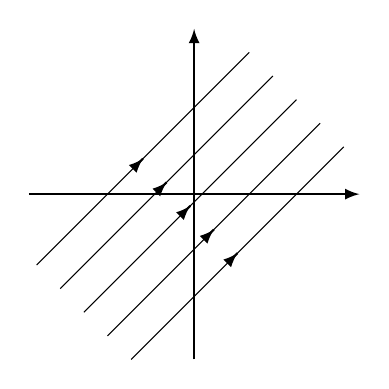
\begin{tikzpicture}
    \draw[black, thick, -latex] (-2.1,0) to (2.1,0);
    \draw[black, thick, -latex] (0,-2.1) to (0,2.1);
    \draw[black] (-2.0, -0.9) to (0.7, 1.8);
    \draw[black, thick, -latex] (-0.65, 0.45) to ++(0.0001,0.0001);
    \draw[black] (-1.7, -1.2) to (1, 1.5);
    \draw[black, thick, -latex] (-0.35, 0.15) to ++(0.0001,0.0001);
    \draw[black] (-1.4, -1.5) to (1.3, 1.2);
    \draw[black, thick, -latex] (-0.05, -0.15) to ++(0.0001,0.0001);
    \draw[black] (-1.1, -1.8) to (1.6, 0.9);
    \draw[black, thick, -latex] (0.25, -0.45) to ++(0.0001,0.0001);
    \draw[black] (-0.8, -2.1) to (1.9, 0.6);
    \draw[black, thick, -latex] (0.55, -0.75) to ++(0.0001,0.0001);
\end{tikzpicture}
}
                \item \resizebox{0.9\columnwidth}{!}{
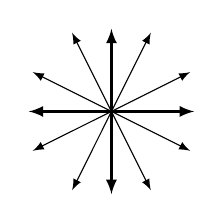
\begin{tikzpicture}
    \draw[black, thick, latex-latex] (-1.05,0) to (1.05,0);
    \draw[black, thick, latex-latex] (0,-1.05) to (0,1.05);
    \draw[black, latex-latex] (-0.5,-1) to (0.5,1);
    \draw[black, latex-latex] (-1,-0.5) to (1,0.5);
    \draw[black, latex-latex] (0.5,-1) to (-0.5,1);
    \draw[black, latex-latex] (1,-0.5) to (-1,0.5);
\end{tikzpicture}
}
                \item \resizebox{0.9\columnwidth}{!}{
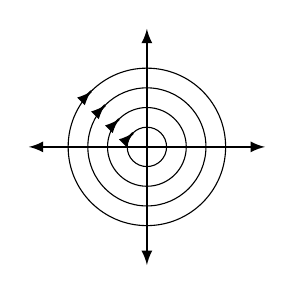
\begin{tikzpicture}
    \draw[black, thick, latex-latex] (-1.5,0) to (1.5,0);
    \draw[black, thick, latex-latex] (0,-1.5) to (0,1.5);
    \draw (0,0) circle (0.25);
    \draw (0,0) circle (0.5);
    \draw (0,0) circle (0.75);
    \draw (0,0) circle (1);
    \draw[black, thick, -latex] (-0.17677669525,0.17677669525) to ++(0.0001,0.0001);
    \draw[black, thick, -latex] (-0.353553391,0.353553391) to ++(0.0001,0.0001);
    \draw[black, thick, -latex] (-0.530330087,0.530330087) to ++(0.0001,0.0001);
    \draw[black, thick, -latex] (-0.707106782,0.707106782) to ++(0.0001,0.0001);
\end{tikzpicture}
}
                \item \resizebox{0.9\columnwidth}{!}{
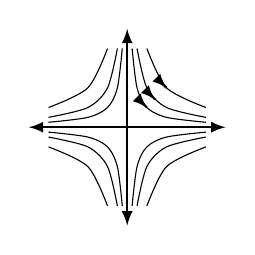
\begin{tikzpicture}
    \draw[black, thick, latex-latex] (-1.25,0) to (1.25,0); 
    \draw[black, thick, latex-latex] (0,-1.25) to (0,1.25); 
    \draw[smooth, variable=\x, black] plot coordinates {(0.25/4, 4/4) (0.5/4, 2/4) (1/4, 1/4) (2/4, 0.5/4) (4/4, 0.25/4)};
    \draw [smooth, variable=\x, black] plot coordinates {(4/4,0.5/4) (2/4,1/4) (1/4,2/4) (0.5/4,4/4)};
    \draw[smooth, variable=\x, black] plot coordinates { (4/4, 1/4) (2/4,2/4) (1/4,4/4)};
    \draw[smooth, variable=\x, black] plot coordinates {(-0.25/4, 4/4) (-0.5/4, 2/4) (-1/4, 1/4) (-2/4, 0.5/4) (-4/4, 0.25/4)};
    \draw [smooth, variable=\x, black] plot coordinates {(-4/4,0.5/4) (-2/4,1/4) (-1/4,2/4) (-0.5/4,4/4)};
    \draw[smooth, variable=\x, black] plot coordinates { (-4/4, 1/4) (-2/4,2/4) (-1/4,4/4)};
    \draw[smooth, variable=\x, black] plot coordinates {(-0.25/4, -4/4) (-0.5/4, -2/4) (-1/4, -1/4) (-2/4, -0.5/4) (-4/4, -0.25/4)};
    \draw [smooth, variable=\x, black] plot coordinates {(-4/4,-0.5/4) (-2/4,-1/4) (-1/4,-2/4) (-0.5/4,-4/4)};
    \draw[smooth, variable=\x, black] plot coordinates { (-4/4, -1/4) (-2/4,-2/4) (-1/4,-4/4)};
    \draw[smooth, variable=\x, black] plot coordinates {(0.25/4, -4/4) (0.5/4, -2/4) (1/4, -1/4) (2/4, -0.5/4) (4/4, -0.25/4)};
    \draw [smooth, variable=\x, black] plot coordinates {(4/4,-0.5/4) (2/4,-1/4) (1/4,-2/4) (0.5/4,-4/4)};
    \draw[smooth, variable=\x, black] plot coordinates { (4/4, -1/4) (2/4,-2/4) (1/4,-4/4)};
    \draw[black, thick, -latex] (1/4,1/4) to ++(0.0001,-0.0001);
    \draw[black, thick, -latex] (2/4,2/4) to ++(0.0001,-0.0001);
    \draw[black, thick, -latex] (1.414/4, 1.414/4) to ++(0.0001,-0.0001);
\end{tikzpicture}
}
            \end{enumerate}
        \end{multicols}
        
\item[] \textbf{Common Data for questions 21 and 22}

Two flat parallel plates are separated by a small gap $h$ filled with an incompressible fluid of viscosity $\mu$. Assume that the length and width of the plates to be much larger than the gap $h$. The top plate moves horizontally while the bottom plate is held stationary. The magnitude of difference between the shear stress at the top and bottom walls is found to be $\Delta\tau$.
    
    \hfill{(2011)}

%3
    \item The velocity of the top plate is

        \begin{multicols}{4}
            \begin{enumerate}
                \item $\frac{h\Delta\tau}{2\mu}$
                \item $\frac{h\Delta\tau}{\mu}$
                \item $\frac{2h\Delta\tau}{\mu}$
                \item $\frac{3h\Delta\tau}{2\mu}$
            \end{enumerate}
        \end{multicols}


%4
    \item If a finite width slender object is introduced parallel to the plates in the middle of the gap, the time at which it would have rotated clockwise by $90\degree$ would be
    
    \hfill{(2011)}
    
	\begin{multicols}{4}
		\begin{enumerate}
                \item $\frac{2\pi\mu}{\Delta\tau}$
                \item $\frac{\pi\mu}{\Delta\tau}$
                \item $\frac{2\pi\mu}{3\Delta\tau}$
                \item $\frac{\pi\mu}{4\Delta\tau}$
			\end{enumerate}
		\end{multicols}

%5
    \item Which of the following pairs of crystal structures can have the same packing fraction of 0.74?
    
    \hfill{(2011)}

    \begin{multicols}{4}
       \begin{enumerate}
            \item FCC and BCC
            \item HCP and BCC
            \item FCC and HCP
            \item BCC and BCT
        \end{enumerate}
    \end{multicols}
  
%6
    \item Which one of the following is NOT CORRECT?
    
    \hfill{(2011)}

    \begin{multicols}{2}
        \begin{enumerate}
            \item An edge dislocation can cross slip
            \item An edge dislocation can glide
            \item A screw dislocation can cross slip
            \item An edge dislocation can climb
        \end{enumerate}
    \end{multicols}

%7
    \item Which of the following is NOT CORRECT?
    
    \hfill{(2011)}


            \begin{enumerate}
                \item Working of lead at $25\degree C$ is hot working
                \item Working of tungsten at $1000\degree C$ is hot working
                \item Working of lead at $-100\degree C$ is cold working
                \item Working of tungsten at $25\degree C$ is cold working
            \end{enumerate}

		
%8
    \item Which one of the following is NOT a ceramic?
    
    \hfill{(2011)}

        \begin{multicols}{4}
            \begin{enumerate}
                \item SiC
                \item MgO
                \item TiB$_2$
                \item TiAl
            \end{enumerate}
        \end{multicols}

%9
    \item If the average degree of polymerization of a polyvinyl chloride (PVC) polymer is 2000, then its average molecular weight (in $\frac{g}{mol}$) is
    
    \hfill{(2011)}

        \begin{multicols}{4}
            \begin{enumerate}
                \item 125000
                \item 119000
                \item 56000
                \item 2000
            \end{enumerate}
        \end{multicols}

%10
    \item Which one of the following materials has the lowest coefficient of thermal expansion?
    
    \hfill{(2011)}

        \begin{multicols}{4}
            \begin{enumerate}
                \item Superalloy
                \item Super Invar
                \item Spinel
                \item $\alpha$-brass
            \end{enumerate}
        \end{multicols}
        
%11
    \item The color of a metal is determined by the wavelength distribution of the radiation that is
    
    \hfill{(2011)}

        \begin{multicols}{4}
            \begin{enumerate}
                \item diffracted
                \item transmitted
                \item reflected
                \item refracted
            \end{enumerate}
        \end{multicols}

%12
    \item Nickel ferrite is
    
    \hfill{(2011)}

        \begin{multicols}{4}
            \begin{enumerate}
                \item antiferromagnetic
                \item ferromagnetic
                \item diamagnetic
                \item ferrimagnetic
            \end{enumerate}
        \end{multicols}
        
%13
    \item The oxide scale responsible for the excellent corrosion resistance of stainless steels is
    
    \hfill{(2011)}

        \begin{multicols}{4}
            \begin{enumerate}
                \item $Cr_2O_3$
                \item $NiO$
                \item $Fe_2O_3$
                \item $Al_2O_3$
            \end{enumerate}
        \end{multicols}

